\documentclass[conference,a4paper]{IEEEtran}
\pdfminorversion=7
\usepackage{cite}
\usepackage{amsmath,amssymb}
\usepackage{booktabs}
\usepackage{graphicx}
\usepackage{microtype}
\usepackage{xcolor}
\usepackage{url}
\newcommand{\loco}{LOCO}
\newcommand{\pressure}{LOP}
\setlength{\textfloatsep}{7pt plus 2pt minus 2pt}
\setlength{\floatsep}{6pt plus 2pt minus 2pt}
\setlength{\intextsep}{6pt plus 2pt minus 2pt}

\title{Beyond Seen Mistakes: Diagnosing Natural Error-Composition\\Shift in Multi-Criterion Exercise Assessment}
\author{\IEEEauthorblockN{Anonymous Author(s)}\\\IEEEauthorblockA{Under double-blind review}}

\begin{document}
\maketitle

\begin{abstract}
Automated exercise assessment predicts several biomechanical criteria at once,
but ordinary grouped evaluation does not directly test a diagnosis composition
chosen to be absent from training. We construct a recording-pair-disjoint
observed-composition holdout protocol on the public ALEX-GYM-1 pose data. The
protocol audits missing detections, excludes one unrecoverable two-view
repetition, and retains 12 natural diagnosis compositions whose training and
validation folds contain both states of every criterion. Across five sequence
models, exact diagnosis match is 11.34 percentage points lower on targeted
leave-one-composition-out tests than on ordinary grouped validation (target
bootstrap 95\% CI $[8.09,14.54]$; two-sided Holm-adjusted $p=.00098$).
We then define Label-Opposition Pressure (LOP), the number of training examples
that match a held-out diagnosis on every other criterion while carrying the
opposite current bit. Within diagnosis, larger LOP is strongly associated with
lower criterion accuracy (raw diagnosis-equal mean Spearman
$\rho=-.651$; 50,000-shuffle blocked $p<.00004$). The result is a reproducible
stress test and a training-label-only diagnostic of natural composition failure,
not a claim of universal architecture superiority or causal label influence.
\end{abstract}

\begin{IEEEkeywords}
exercise assessment, multi-label classification, compositional generalization,
skeleton sequences, label-space diagnostics
\end{IEEEkeywords}

\section{Introduction}
Fine-grained exercise assessment differs from ordinary action recognition. A
system must report several simultaneous errors---for example foot orientation,
hip position, back posture, and movement depth---rather than one action class.
Consequently, a label is a binary diagnosis vector
$\mathbf y\in\{0,1\}^{C}$, and the practically relevant question is whether
individually familiar criterion states remain recognizable when they occur in a
new combination.

The distinction is easy to miss. A recording-disjoint random split protects
against direct source overlap, but it does not deliberately hold out a chosen
diagnosis vector. A model can therefore obtain reasonable marginal accuracy
while using pose patterns correlated with entire diagnoses. This matters for
feedback: one systematically wrong criterion invalidates an otherwise plausible
diagnosis.

Composite errors have been studied directly by CPR-Coach, which trains on
isolated error classes and tests synthetically enumerated composites
\cite{wang2024cpr}. Held-out label combinations are also established in
multi-label learning \cite{chai2024compositional}. Our setting is narrower and
naturalistic: training remains multi-error, every evaluated criterion state has
training support, and test diagnoses are naturally observed in a public
two-view exercise dataset. We do not claim the first composite-error task or the
first combination split.

We organize the study around two retrospective research questions. \textbf{RQ1}
asks whether ordinary grouped validation hides failure on a diagnosis deliberately
absent from training. \textbf{RQ2} asks whether the local training-label
neighborhood identifies the vulnerable criteria. Because these
questions were fixed after an initial repository audit rather than preregistered,
all primary tests are two-sided and Holm-corrected.

We contribute a data-audited, recording-pair-disjoint observed-composition
protocol with explicit feasibility rules and a frozen split manifest. We also
introduce a training-label-only opposition statistic that strongly localizes
criterion failure within held-out diagnoses. Figure \ref{fig:protocol} shows the
sparse, naturally observed diagnosis spaces and the targets retained by the final
support rule.

\begin{figure*}[t]
\centering
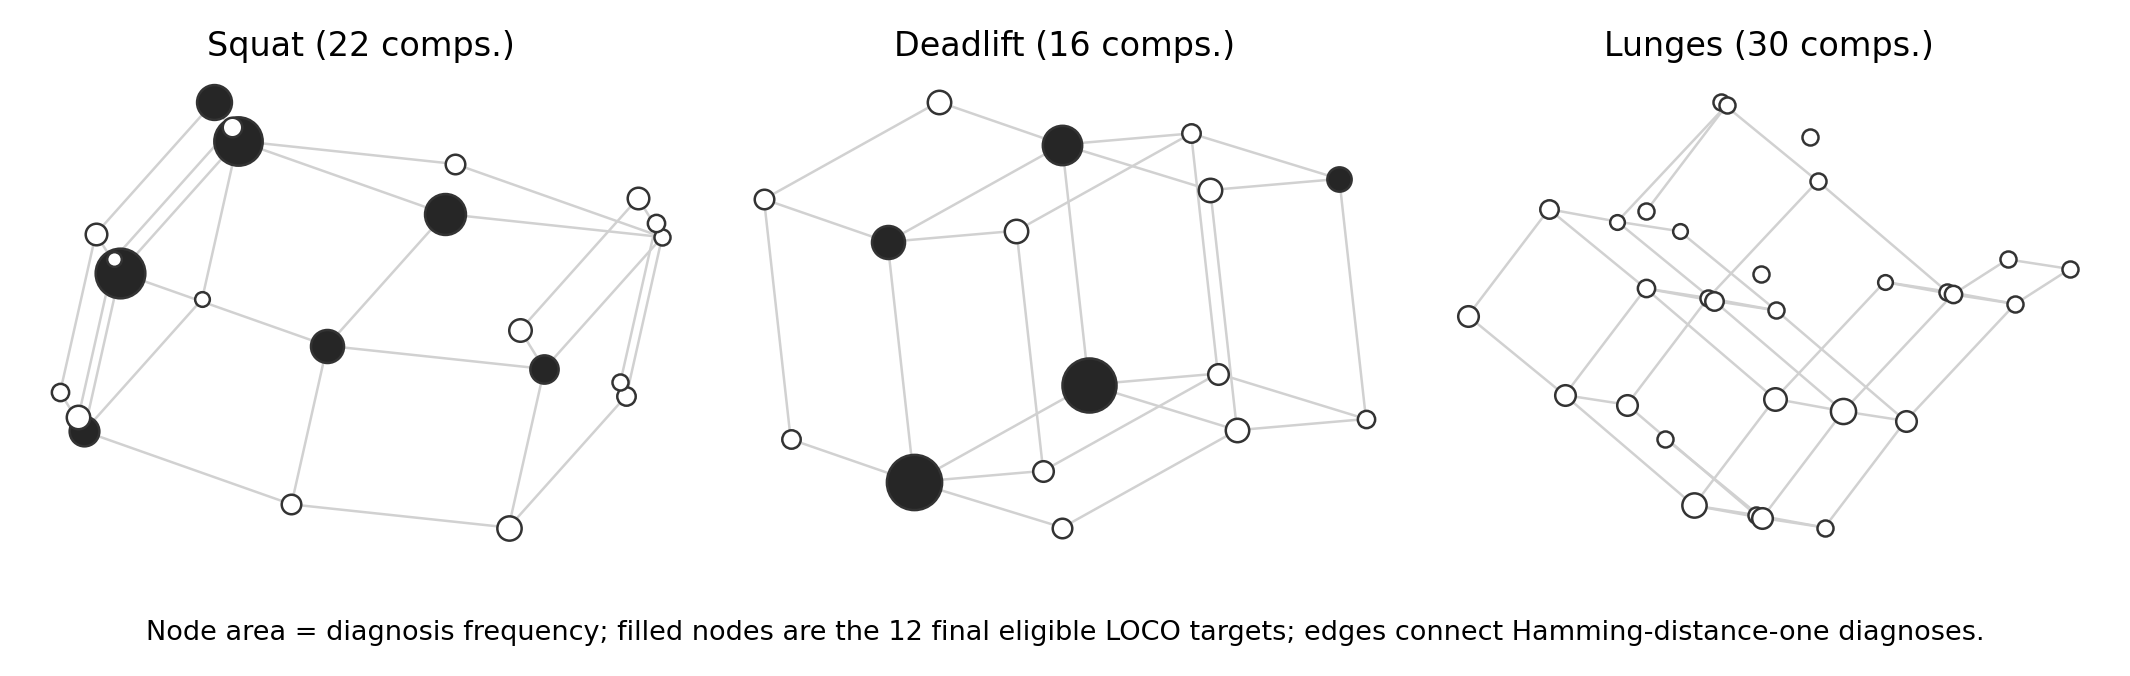
\includegraphics[width=.98\textwidth]{figures/composition_graph.png}
\caption{Naturally observed diagnosis spaces. Node area represents repetition
frequency, filled nodes are the 12 targets retained by the final support rule,
and edges join diagnoses differing in exactly one criterion. Lunge has no filled
node because its candidate targets cannot preserve the required train/validation
state support after recording-group removal.}
\label{fig:protocol}
\end{figure*}

\section{Related Work}
\subsection{Exercise assessment and composite errors}
ALEX-GYM-1 provides two-view 3D poses and multi-criterion exercise annotations
\cite{hassan2025alexgym}. Other rehabilitation datasets emphasize clinical scores,
correctness, or multi-task assessment rather than natural held-out multi-error
label sets \cite{capecci2019kimore,vakanski2018uiprmd,li2024finerehab}.
FineDiving and FineParser study procedure-aware action quality at fine temporal
granularity \cite{xu2022finediving,xu2024fineparser}, but not this diagnosis-set
shift. CPR-Coach is the closest direct composition formulation
\cite{wang2024cpr}; its isolated-error training regime differs from our naturally
multi-error training pool.

Learnable Motion-Focused Tokenization (LMFT) drops low-motion RGB patches to
reduce background-driven video domain shift \cite{liu2026lmft}. Our normalized
pose input contains no scene background, while static joint configurations can
define form errors. LMFT is therefore an adjacent evidence-selection principle,
not a directly matched method or baseline for diagnosis-composition shift.

\subsection{Multi-label shortcuts and unseen combinations}
Multi-label models often exploit label dependence. Compositional multi-label
classification explicitly holds out label combinations \cite{chai2024compositional},
while counterfactual and correlation-shortcut work studies harmful co-occurrence
dependence \cite{xie2024counterfactual,fan2023cftc}. We use this literature to
motivate a diagnostic, not a causal claim: label counts characterize exposure in
the benchmark and never enter the exercise classifier.

\section{Data and Protocol}
\subsection{Dataset and preprocessing audit}
The public ALEX-GYM-1 subset contains squat, Romanian deadlift, and lunge
repetitions with frontal and lateral 33-joint 3D pose sequences. We convert each
trainer criterion to an error bit: one denotes a violated criterion. Table
\ref{tab:data} summarizes the processed data.

\begin{table}[t]
\centering
\caption{Processed ALEX-GYM-1 data. ``Groups'' are paired recording identifiers,
not verified participant identities.}
\label{tab:data}
\small
\begin{tabular}{lrrrr}
\toprule
Exercise & Repetitions & Criteria & Diagnoses & Groups\\
\midrule
Squat & 294 & 6 & 22 & 59\\
Deadlift & 269 & 5 & 16 & 55\\
Lunge & 106 & 7 & 30 & 53\\
\bottomrule
\end{tabular}
\end{table}

All-zero frames occur in both views: squat has 183/4,720 frontal (3.88\%) and
702/4,720 lateral frames (14.87\%); deadlift has 250/4,304 (5.81\%) and
326/4,304 (7.57\%); and lunge has 33/1,696 (1.95\%) and 214/1,696 (12.62\%),
respectively. We linearly
interpolate whole missing frames before pelvis centering, robust body-scale
normalization, and resampling to 16 frames. One squat repetition has no valid
frontal frame and is excluded. Raw-file SHA-256 hashes, the exclusion, and
per-sequence quality counts are released. We do not impute isolated zero joints,
whose semantics cannot be verified from the release.

\subsection{Observed-composition holdout}
For exercise $e$, let $s_i$ identify a paired frontal/lateral recording and
$\mathbf y_i$ its diagnosis. For target diagnosis $\mathbf y^*$, the test set is
all repetitions with $\mathbf y_i=\mathbf y^*$. Every recording group containing
that target is removed from the train/validation pool, including its non-target
repetitions. The remaining groups are split deterministically. Candidate splits
are rejected unless both states of every criterion occur at least eight times in
training and at least once in validation. Train--validation, train--test, and
validation--test group intersections are zero in every fold.

A target is eligible when it has at least ten repetitions, three source groups,
and a feasible supported split. Seven squat and five deadlift diagnoses qualify.
Two lunge diagnoses considered by the earlier protocol are infeasible: their
minority pool contains exactly eight examples, so eight cannot remain in training
while one also enters validation. They are excluded rather than evaluated under a
different rule. The primary experiment is therefore 12 targets $\times$ three
seeds per model.

The comparator is ordinary recording-group validation, not a guaranteed
seen-composition set: 409 of 1,760 validation rows (23.2\%) have a diagnosis absent
from that fold's training subset. RQ1 consequently measures ordinary grouped
validation versus a \emph{targeted} composition stress test; it does not attribute
the entire gap solely to seen/unseen status.

\subsection{Models and training}
We use five compact controlled models: a temporal CNN, BiGRU, Transformer,
selective state-space model, and Factorized Anatomical Criterion Tokens (FACT).
All baselines receive a $16\times198$ sequence (two views $\times$ 33 joints
$\times$ xyz). The TCN uses a 96-D frame embedding, temporal kernels 5 and 3,
and mean/max pooling. BiGRU uses a 72-D bidirectional GRU; Transformer uses two
96-D, four-head encoder layers; and SSM uses one 32-D bidirectional selective
scan. Their deadlift models contain 112k, 99k, 190k, and 13k parameters,
respectively. The SSM is a compact study implementation rather than an official
reproduction of a named large model.

FACT reshapes each sequence to $2\times16\times33\times3$. For criterion $c$,
the annotation wording specifies one view and an initial joint set. A learned
residual adjusts a sigmoid mask initialized near .95 on mapped joints and .05
elsewhere. Separate frontal/lateral encoders apply a 56-D frame projection,
temporal convolutions of width 5 and 3, and mean/max pooling. A criterion-specific
$112\!\rightarrow\!32$ adapter produces one token per criterion. Its logit sums
a local linear score and a scaled distance difference to two learned 32-D state
prototypes. FACT never consumes other labels or logits at inference and contains
84,858 parameters for squat and 81,048 for deadlift. It is a locality-oriented
comparator, not a claimed generally superior architecture.

Every model receives the same normalized two-view representation and split.
Models use class-weighted binary cross-entropy, AdamW, fixed 0.5 thresholds, and
early stopping on validation macro-F1. Hyperparameters are never selected using
the held-out target. We report target-equal means: seeds are averaged within
target, then all 12 targets receive equal weight. All primary trainers call the
same deterministic constrained splitter. The released manifest records raw-file
hashes, preprocessing version, exact indices, target support, exclusions, and
zero group intersections for every target and seed.

\section{Label-Space Diagnostic}
\subsection{Label-Opposition Pressure}
For criterion $c$, let $\mathbf y^*_{-c}$ denote the other criterion bits. Label-
Opposition Pressure is
\begin{equation}
\pressure_c(\mathbf y^*)=\sum_{i\in\mathcal T}
\mathbb 1[\mathbf y_{i,-c}=\mathbf y^*_{-c}]
\mathbb 1[y_{i,c}\ne y_c^*],
\end{equation}
where $\mathcal T$ is the fold training set. Large pressure means many training
examples reproduce the target context while supporting the wrong current bit.
LOP is an exposure association, not causal influence or deployment confidence.

\section{Statistical Analysis}
The held-out diagnosis is the statistical unit. For RQ1, we average each metric
over seeds and models within target, then test the 12 validation--LOCO differences.
Exact match is primary; bit accuracy is secondary. For RQ2, we average TCN and
FACT criterion accuracy over seeds, compute Spearman correlation within each
diagnosis, and take the raw diagnosis-equal mean across the 12 informative
diagnoses (seven contain six criteria and five contain five). A 50,000-shuffle
test permutes pressure only among criteria of the same diagnosis. This blocked
randomization retains within-diagnosis dependence and calibrates the chosen raw
mean statistic without a parametric correlation assumption.

Both reported primary tests are two-sided. To avoid improving significance by
removing a null result after inspection, their reported Holm values retain the
original three-test family: the third audited analysis, a validation-fitted
label-neighborhood deferral score, was inconclusive overall ($p=.092$) and is
released as supplementary analysis rather than promoted as a contribution. We
report 100,000-sample target bootstrap intervals.

\section{Results}
\subsection{RQ1: targeted composition testing exposes exact-diagnosis failure}
Figure \ref{fig:protocol} summarizes the target-level comparison. Averaged over models,
ordinary grouped validation exceeds targeted LOCO exact match by 11.34 points
(95\% CI $[8.09,14.54]$; two-sided Wilcoxon $p=.00049$, Holm $p=.00098$).
Thus RQ1 is supported for its primary endpoint. Bit accuracy falls by 4.61 points
(CI $[0.25,9.74]$), but its two-sided $p=.151$ is not significant.

Table \ref{tab:models} shows that FACT has the largest mean bit accuracy and exact
match, but its advantage over TCN is unresolved: $+1.85$ bit points ($p=.204$)
and $+2.75$ exact points ($p=.086$) in two-sided exploratory comparisons. We
therefore make no architecture-superiority claim. Table \ref{tab:models} reports
micro-F1 pooled across criterion decisions. Macro-F1 is omitted because every
criterion has one constant state inside a target fold; fold-level macro-F1 is
not a meaningful discrimination measure in this protocol. ``Bit'' is the
fraction of all criterion decisions that are correct; ``Exact'' requires every
criterion of a repetition to be correct. Thus FACT's 64.89 LOCO Bit but 5.14
Exact means that 64.89\% of individual decisions are correct while only 5.14\%
of complete diagnosis vectors are correct.

\begin{table}[t]
\centering
\caption{Target-equal performance (\%). Validation is ordinary group-held-out;
LOCO deliberately withholds one natural diagnosis.}
\label{tab:models}
\scriptsize
\setlength{\tabcolsep}{3.2pt}
\begin{tabular}{lrrrrrr}
\toprule
& \multicolumn{3}{c}{Validation} & \multicolumn{3}{c}{LOCO}\\
Model & Bit & $\mu$F1 & Exact & Bit & $\mu$F1 & Exact\\
\midrule
TCN & 65.08 & 56.35 & 12.61 & 63.04 & 44.86 & 2.39\\
BiGRU & 65.32 & 57.00 & 14.71 & 60.61 & 42.11 & 2.63\\
Transformer & 64.26 & 57.08 & 12.20 & 59.83 & 41.79 & 2.07\\
Selective SSM & 66.89 & 56.91 & 14.23 & 62.50 & 41.82 & 3.41\\
FACT & \textbf{72.39} & \textbf{63.95} & \textbf{18.56} & \textbf{64.89} & 44.77 & \textbf{5.14}\\
\bottomrule
\end{tabular}
\end{table}

\subsection{RQ2: the one-bit label neighborhood localizes failure}
Across 67 target--criterion units, LOP and held-out accuracy are negatively
related within target. The raw diagnosis-equal mean Spearman correlation is
$-.651$. The diagnosis-blocked two-sided permutation probability is
$p<.00004$ (Holm $p=.00012$), supporting RQ2. Figure \ref{fig:pressure} shows the
corresponding error trend. Because criteria within a diagnosis share samples and
predictions, a pooled row-level parametric test would be anticonservative; the
blocked permutation is the primary inference.

\begin{figure}[t]
\centering
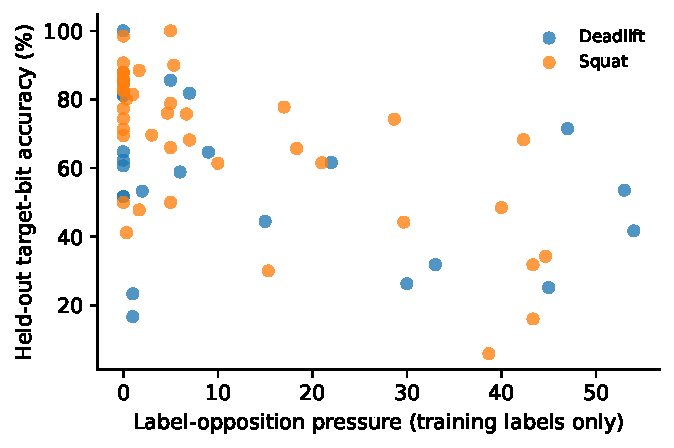
\includegraphics[width=\columnwidth]{figures/rq2_pressure_error.pdf}
\caption{One-bit training-label opposition versus LOCO criterion error for the
TCN/FACT anchor analysis. Points are seed- and model-averaged target--criterion
units; the line is descriptive.}
\label{fig:pressure}
\end{figure}

\section{Discussion}
The strongest result is not that a particular backbone wins; it is that exact
multi-criterion diagnoses fail under a targeted natural composition stress test
even when all criterion states retain training support. Marginal bit accuracy can
hide this effect, explaining why its secondary gap is much smaller and
statistically unresolved.

LOP supplies a simple account of which bit fails. If many training diagnoses
match the held-out context but contain the opposite value of criterion $c$, a
learner can associate the surrounding movement with the wrong bit. This remains
an association: the classifier never consumes ground-truth co-labels at
inference, and pose features may encode the same correlations.

\section{Limitations}
The study has one multi-label composition dataset and only 12 eligible diagnosis
units. The split key identifies paired recordings, not verified participants, so
we claim recording-pair rather than participant separation. Validation is not a
pure seen-composition control. Manual criterion--anatomy mappings affect FACT,
which is why FACT is only a comparator. Thresholds are fixed at 0.5, and no claim
is made about calibrated probabilities. Missing-frame rates reach 14.87\%
in the squat lateral view; interpolation reduces but cannot eliminate uncertainty
from pose-detector failures. Finally, exact match is clinically
intuitive but harsh; it is reported alongside bit accuracy and micro-F1.

\section{Conclusion}
Natural exercise diagnoses are more than collections of familiar bits. Under a
recording-pair-disjoint observed-composition protocol, exact diagnosis match falls
sharply relative to ordinary grouped validation. A one-bit training-label
opposition statistic strongly identifies vulnerable criteria within diagnosis.
The resulting contribution is a reproducible stress test and an honest
label-space diagnostic, with clear evidence about both utility and limits.

\IEEEtriggeratref{6}
\begin{thebibliography}{99}
\bibitem{hassan2025alexgym} A. Hassan, A. Serour, A. Gamea, and W. Gomaa,
``ALEX-GYM-1: A novel dataset and hybrid 3D pose vision model for automated
exercise evaluation,'' in \emph{Proc. ICINCO}, 2025, pp. 24--34.

\bibitem{wang2024cpr} J. Wang \emph{et al.}, ``CPR-Coach: Recognizing composite
error actions based on single-class training,'' in \emph{Proc. IEEE/CVF CVPR},
2024.

\bibitem{chai2024compositional} Y. Chai \emph{et al.}, ``Compositional
generalization for multi-label text classification,'' in \emph{Proc. AAAI},
2024.

\bibitem{capecci2019kimore} M. Capecci \emph{et al.}, ``The KIMORE dataset:
Kinematic assessment of movement and clinical scores for remote monitoring of
physical rehabilitation,'' \emph{IEEE Trans. Neural Syst. Rehabil. Eng.}, 2019.

\bibitem{vakanski2018uiprmd} A. Vakanski, H. Jun, D. Paul, and R. Baker, ``A
data set of human body movements for physical rehabilitation exercises,''
\emph{Data}, vol. 3, no. 1, 2018.

\bibitem{li2024finerehab} J. Li \emph{et al.}, ``FineRehab: A multi-modality and
multi-task dataset for rehabilitation analysis,'' in \emph{Proc. IEEE/CVF CVPR
Workshops}, 2024.

\bibitem{xu2022finediving} J. Xu \emph{et al.}, ``FineDiving: A fine-grained
dataset for procedure-aware action quality assessment,'' in \emph{Proc. IEEE/CVF
CVPR}, 2022.

\bibitem{xu2024fineparser} J. Xu \emph{et al.}, ``FineParser: A fine-grained
spatio-temporal action parser for human-centric action quality assessment,'' in
\emph{Proc. IEEE/CVF CVPR}, 2024.

\bibitem{xie2024counterfactual} B. Xie \emph{et al.}, ``Counterfactual
multi-label learning,'' in \emph{Proc. ICML}, 2024.

\bibitem{fan2023cftc} Z. Fan \emph{et al.}, ``CFTC: Combating label correlation
shortcut in multi-label classification,'' arXiv:2310.07588, 2023.

\bibitem{liu2026lmft} T. L. Liu, I. Stavness, and M. Rochan, ``Learnable
motion-focused tokenization for effective and efficient video unsupervised
domain adaptation,'' in \emph{Proc. IEEE/CVF CVPR}, 2026.

\end{thebibliography}
\end{document}
